\section{The Large Hadron Collider}
\label{sec:lhc}

The LHC~\cite{LHCMachine} is a circular particle accelerator, with a 27~kilometer circumference,
located at an average distance of 100 meters beneath the surface of the Earth.
It is nominally used for proton-proton ($pp$) collisions, wherein two counter-rotating
beams of protons are made to collide head-on at specific interaction points (IP) along the 27~kilometer
ring, but can also be run in heavy-ion configurations wherein proton-lead ($p$-Pb) or lead-lead (Pb-Pb)
collisions take place.\footnote{More rarely, the LHC can also be used to circulate gold (Au) ions.
There are even plans to have proton-oxygen ($p$-O) runs in the future, which will allow
for the LHC experiments to provide research that potentially complements dark matter research
based on cosmic-ray air showers.}
{\color{red}{what specific Pb ion?}}
The $pp$ collisions take priority over those of the heavy-ions, with the collisions each year
consisting of only a few weeks in the winter for the heavy-ion configurations and typically
six to seven months for the $pp$ configuration. The LHC is designed to accelerate protons to a
center-of-mass energy of $\sqrt{s} = 14\,\TeV$.

%\subsection{Keeping the Protons In Line}
\paragraph{Keeping the Protons in Line} \mbox{} \\
\label{sec:dipole}

The LHC was planned as the successor to the Large Electron Positron (LEP) collider, which was in operation
between the years of 1989 to 2000. LEP is still the most powerful lepton collider to date, having maximal electron-positron
center-of-mass collision energies of 209\,\GeV.
After LEP, the particle physics community knew that the next collider needed to have multi-\TeV~collision
energies; either to be able to probe from all angles any new physics discovered at LEP, or
to provide the necessary power to search for still-elusive hints of BSM physics. At the very least,
given a non-discovery of the Higgs boson at LEP, the community would need a discovery machine powerful enough
to produce electroweak-scale Higgs bosons and a multi-\TeV~hadron collider --- as we now know --- is sufficient for this job.


%The LHC~\cite{LHCMachine} is a circular particle accelerator with a 27~kilometer circumference
%located at an average distance of 100 meters beneath the Earth's surface.
%It is nominally used for proton-proton ($pp$) collisions, wherein two counter-rotating
%beams of protons are made to collide head-on at specific interaction points (IP) along the 27~kilometer ring,
%but can also be run in heavy-ion configurations, such as proton-lead ($p$-Pb) or lead-lead (Pb-Pb)
%collisions. The $pp$ collisions for the most part take priority over those of the heavy-ions,
%and the yearly data-taking period only a few weeks in the winter are typically allocated for
%heavy-ion configurations whereas six to seven months can be allocated for the $pp$ configuration.

%The LHC~\cite{Evans_2008} is a circular particle accelerator with a 27~kilometer ($\approx17$ miles)
%circumference located, on average, approximately 100 meters beneath the Earth's surface. It is nominally
%a proton-proton ($pp$) collider
%but can also be run in heavy-ion configurations: proton-lead ($p$-Pb), lead-lead (Pb-Pb), or even
%proton-gold ($p$-Au). It is designed to accelerate protons to a center-of-mass
%energy of $\sqrt{s} = 14\,\TeV$.

In order to increase center-of-mass collisions energies, collider designs can take two routes: they can
either be larger, that is, have larger circumferences (radii), or they can increase the strength of the magnetic
fields used to keep the circulating charged particles in orbit. This can be seen by considering the expression
for the relativistic cyclotron frequency, $\omega$, of a particle moving in a circular orbit,
\begin{align}
    \omega = \frac{qB}{\gamma m},
    \label{eq:rel_cyclotron}
\end{align}
where $m$ is the particle's rest mass, $B$ is the magnitude of the magnetic field experienced by the
particle, $q$ is the particle's electric charge, and $\gamma$ is the relativistic Lorentz factor, $\gamma = \sqrt{1 - \beta^2} = \sqrt{1 - (v/c)^2}$,
with $v$ the particle's velocity and $c$ the speed of light. A particle of higher energy confined
to a fixed circular orbit necessarily has a higher
angular velocity, which can be seen by the expression relating the angular velocity to kinetic energy:
\begin{align}
    E_{\text{kin}} \propto m v^2 = m(\omega R)^2 = \frac{q^2 B^2 R^2}{m \gamma^2}.
    \label{eq:kinetic_energy_gen}
\end{align}
In planning the construction of the LHC, the costs in civil engineering and real-estate works that would
be required to construct a larger tunnel in which to house the LHC ring (increasing $R$) far outweighed
the costs of research into and development of magnet systems strong enough to bend the
multi-\TeV~particles along the beam orbit prescribed by the already-existing LEP tunnel (increasing $B$).
The desired multi-\TeV~center-of-mass collision energy, the fact that the LHC would be a hadron (proton)
collider, and the fact that the LHC would be using the existing LEP tunnel dictate the required magnetic
field strength needed to keep the protons in stable orbits. This
is seen by using Eqn.~\ref{eq:kinetic_energy_gen}, solving for $B$, and comparing the LHC and LEP
design parameters,
\begin{align}
    \hspace{-0.4cm}
    \frac{B^2_{\text{LHC}}}{B^2_\text{LEP}} &= \frac{ (E_{\text{LHC}} m_{\text{LHC}} \gamma_{\text{LHC}}^2) / (q_{\text{LHC}}^2 R_{\text{LHC}}^2)  } { (E_{\text{LEP}} m_{\text{LEP}} \gamma_{\text{LEP}}^2) / (q_{\text{LEP}}^2 R_{\text{LEP}}^2) } \label{eq:lhc_mag_field} \\
        &= (E_{\text{LHC}} / E_{\text{LEP}}) \times (m_{\text{LHC}} / m_{\text{LEP}}) \times (\gamma_{\text{LHC}}^2 / \gamma_{\text{LEP}}^2) \times (q_{\text{LEP}}^2 / q_{\text{LHC}}^2) \times (R_{\text{LEP}}^2 / R_{\text{LHC}}^2) \notag \\
        &\approx ( 1\,\TeV~/0.2\,\TeV) \times (m_p/ m_e) \times (1) \times (1) \times (1) \notag \\
        &\approx 10^4 \notag,
\end{align}
which shows that the strength of the LHC bending magnets must be on the order of $100\times$
the strength of those used at LEP. The magnetic fields experienced by the electron and positron beams
at LEP were 0.22 Tesla. By Eqn.~\ref{eq:lhc_mag_field}, the LHC bending magnets should achieve magnetic field
strengths on the order of 10 Tesla in order to achieve the desired multi-\TeV~center-of-mass collision energies.
The maximum achievable magnetic field of conventional ferrormagnets is about 2 Tesla.
To meet the $\sqrt{s}\approx$10\,\TeV~design goal, the entirety of the magnet system used by the LHC to confine the protons to their circular orbits
must then be composed of \textit{superconducting} electromagnets. %\footnote{Note that even though
%the main dipole bending magnets at LEP were not superconducting, its focusing quadrupole magnets
%\textit{were} superconducting. There are simply fewer quadrupole magnets, as compared to the number of
%dipole magnets, required for a particle collider.}
All of the bending and focusing magnets at the LHC, then, are submerged in a bath of superfluid Helium
at a temperature of $1.9$\,K to keep them in the superconducting state. In total, the LHC contains more than 120 tonnes of superfluid Helium.

Additionally, the fact that LEP was a \textit{particle-antiparticle} collider meant that the counter-rotating
beams could be made to occupy a single ring: the same magnetic field could produce counter-rotating beams of
electrons and positrons within the same beam pipe.\footnote{The electrons and positrons at LEP were vertically separated
within the beam pipe by electrostatic separators placed throughout the LEP ring. Turning off these separators
is, to first approximation, how the LEP operators would get the electrically attracting electrons and positrons to collide.}
As a result, the LEP beam tunnel was constructed with only a single ring in mind and is relatively narrow: the LEP tunnel,
and therefore LHC tunnel, is only $\approx3.7$\,m wide on average.
As the LHC is a \textit{particle-particle} collider, it necessarily requires \textit{two} magnetic fields
of opposing polarity to circulate one of its beams in the clockwise direction and the other in the
counter-clockwise direction.
Given the limited space in the tunnel, however, it is not possible to house two separate rings
of superconducting bending magnets, with all of the services that they require \textit{in addition} to the requisite
minimal space needed for personnel and maintenence access.
This forced the need of the so-called ``2-in-1'' design of the main bending magnets of the LHC, wherein the two
beam pipes are housed in the same cryostat in which the counter-rotating beams are held in their
respective orbits by coupled magnetic fields.
An illustration of this now-iconic design of the LHC magnets is illustrated in Figure~\ref{fig:lhc_dipole_xsec}.
Each of the 15\,meter long superconducting dipole electromagnets of the LHC responsible for constraining the protons to their circular
orbits has currents of $11850$\,Amperes flowing through it and achieves magnetic field strengths of $8.3$\,Tesla.

\begin{figure}[!htb]
    \begin{center}
        \begin{minipage}{\textwidth}
        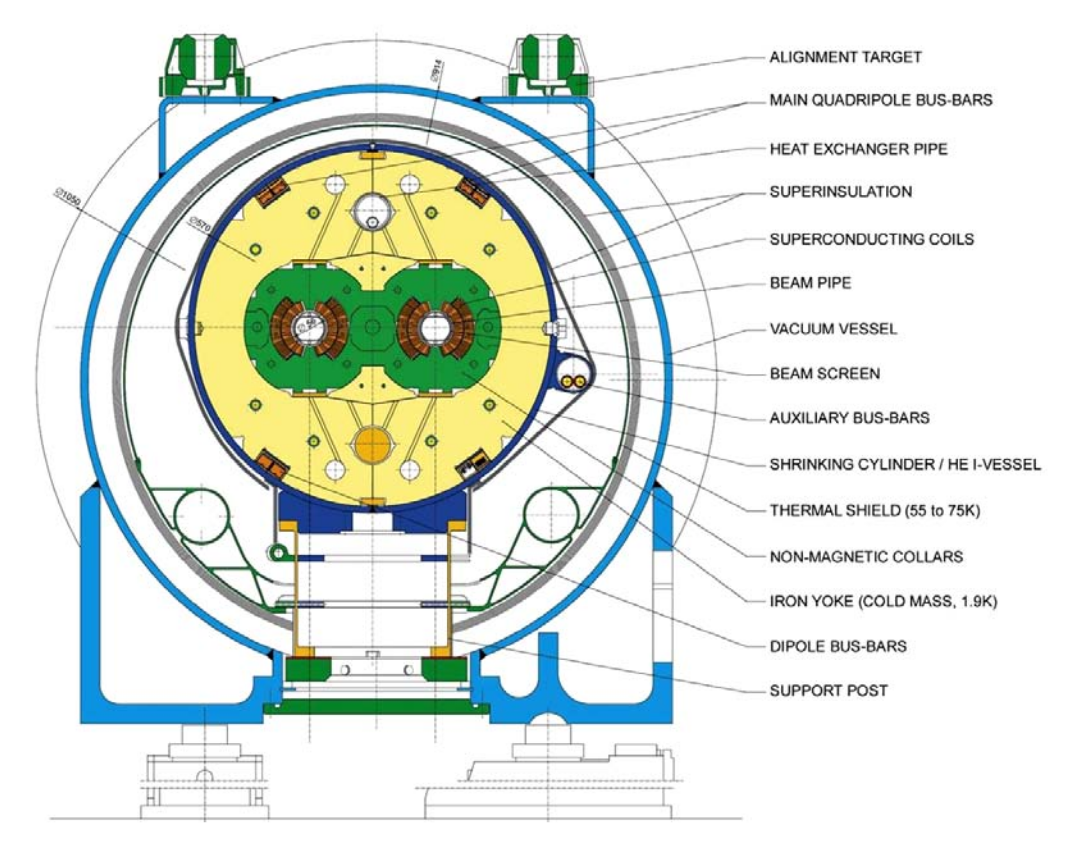
\includegraphics[width=0.59\textwidth]{figures/chapter2/lhc_dipole_fig3p3}
        \raisebox{0.5cm}{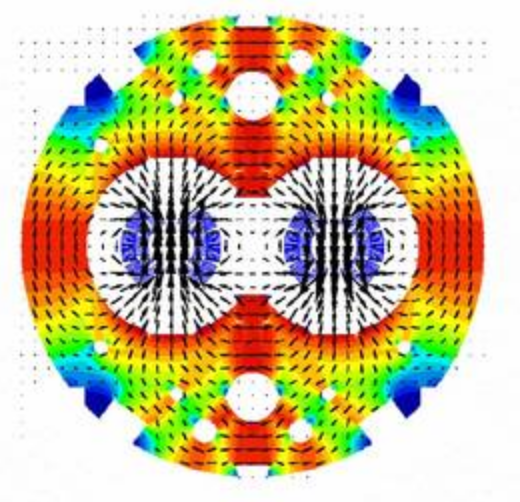
\includegraphics[width=0.4\textwidth]{figures/chapter2/dipole_magnetic_field_lines}}
        \end{minipage}
        \caption{
            \textit{Left}: Cross-sectional view of an LHC dipole bending magnet, with relevant parts indicated.
            \textit{Right}: Magnetic field lines of the coupled dipole fields that bend the counter-rotating proton beams
            and keep them in their circular orbits around the LHC ring.
        }
        \label{fig:lhc_dipole_xsec}
    \end{center}
\end{figure}

\paragraph{Connecting the Dots} \mbox{} \\

Now that we have an idea of the components that make up the LHC ring itself and how it keeps proton beams in stable
orbits, we can take a step back and get an idea of the overall layout of the LHC.
In Figure~\ref{fig:lhc_layout} we see an illustration of the LHC design.
There are...

As shown in Figure~\ref{fig:lhc_layout}, the LHC is comprised of 8 straight sections and 8 curved sections.

\begin{figure}[!htb]
    \begin{center}
        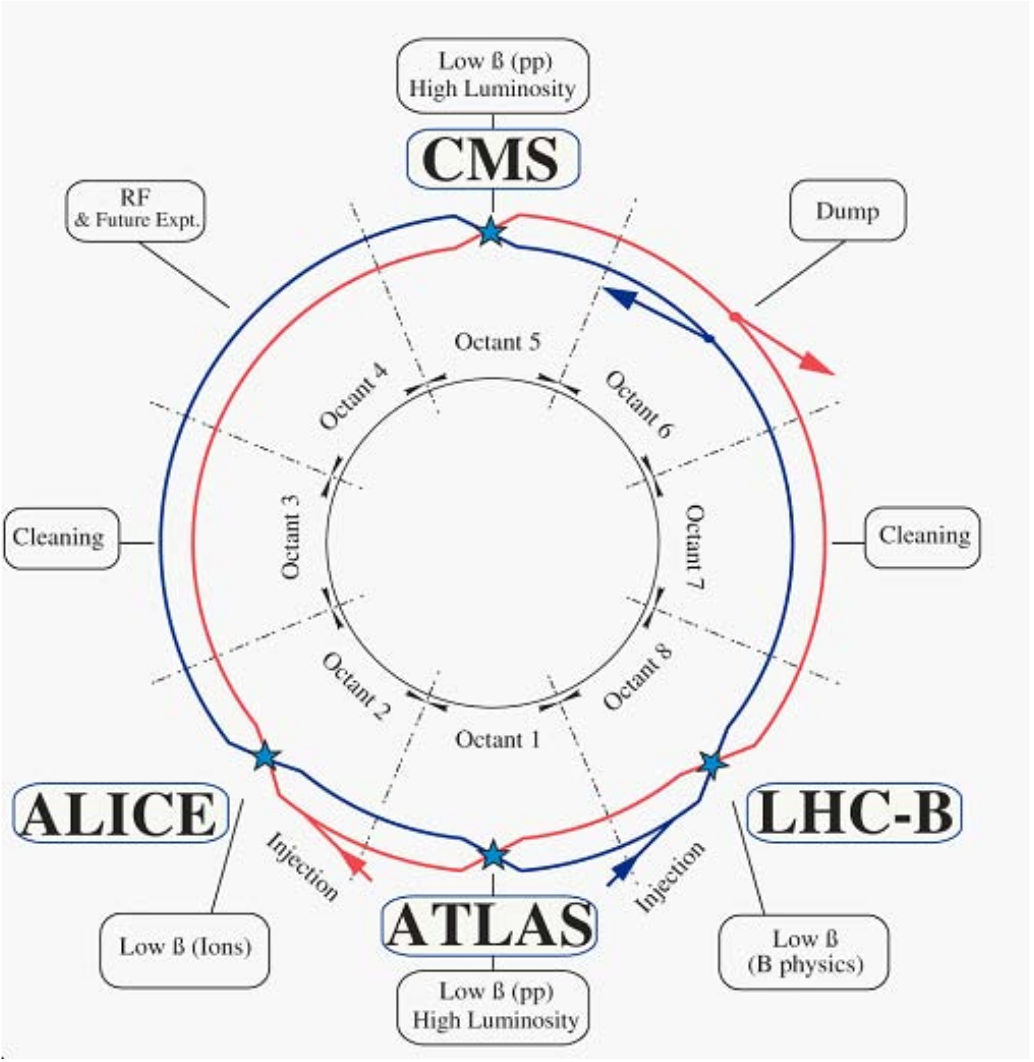
\includegraphics[width=0.8\textwidth]{figures/chapter2/lhc_layout}
        \caption{
            Layout of the LHC and its two counter-rotating beams. Beam 1 is in blue and rotates
            counter-clockwise. Beam 2 is in red and rotates clock-wise.
            At the center of each octant is a straight section which houses
            the experimental caverns or LHC beam facilities.
            At the boundaries of each octant are located the curved sections.
            Figure taken from Figure 2.1 of Ref.~\cite{LHCMachine}.
            {\color{red}{Somewhere $\beta$ should be described -- betatron function}}
        }
        \label{fig:lhc_layout}
    \end{center}
\end{figure}

\FloatBarrier
\subsection{Injection Chain}
\label{sec:lhc_injection}

\subsection{LHC Beam Acceleration and Structure}
\label{sec:lhc_acceleration}

\subsection{The Concept of Luminosity}
\label{sec:lhc_luminosity}

{\color{red}{tabulated design parameters of LHC}}
